%%%%%%%%%%%%%%%%%%%%%%%%%%%%%%%%%%%%%%%%%
% Beamer Presentation
% LaTeX Template
% Version 1.0 (10/11/12)
%%%%%%%%%%%%%%%%%%%%%%%%%%%%%%%%%%%%%%%%%
%----------------------------------------------------------------------------------------
%	PACKAGES AND THEMES
%----------------------------------------------------------------------------------------
\documentclass[aspectratio=169]{beamer}
\mode<presentation> {
\usetheme{Madrid}
}

\usepackage{graphicx} % Allows including images
\usepackage{booktabs} % Allows the use of \toprule, \midrule and \bottomrule in tables
\usepackage{multicol}
\usepackage{multirow}
\usepackage{longtable}
\usepackage[utf8]{inputenc}
\usepackage{enumerate}
\usepackage{color,url}
% ########## user defined
\usepackage{tikz}
\usetikzlibrary{patterns}
\usepackage{calc}
\usepackage{subfig}
\usepackage{pgfplots}
\pgfplotsset{compat=1.9}
\usepackage{pgf-pie}
\usepackage{algorithm}
\usepackage{algpseudocode}
\usepackage{listings}
\lstset{language=Python,basicstyle=\ttfamily,keywordstyle=\color{blue}}
\usepackage{caption}

\AtBeginSection[]{
  \begin{frame}
  \vfill
  \centering
  \begin{beamercolorbox}[sep=8pt,center,shadow=true,rounded=true]{title}
    \usebeamerfont{title}\insertsectionhead\par%
  \end{beamercolorbox}
  \vfill
  \end{frame}
}


%----------------------------------------------------------------------------------------
%	TITLE PAGE
%----------------------------------------------------------------------------------------
\title{Tempus}
\subtitle{Sistemas de Informação 2026-1}

\author[Carlos, Thomas, Gabriel B, Bruno, Gabriel A, Mike]{
Carlos Cauã - 231034304; Thomas Jefferson - 202033561
\newline
Gabriel Bismarck - 170103323; Bruno Gabriel - 241022460
\newline
Gabriel Alexandre - 241038942; Mike Dantas - 140064338
}

\institute[UnB]{Graduação em Ciência da Computação \\ 
    \medskip
    {
\includegraphics[scale=.25]{logo-unb}}
    \medskip
    \date{August 25, 2022}}% Date, can be changed to a custom date

\begin{document}

\begin{frame}
\titlepage
\end{frame}

% Sumário
\begin{frame}
\frametitle{Sumário}
\tableofcontents
\end{frame}

%------------------------------------------------
\section[Ideia Central]{Ideia Central}
%------------------------------------------------

\begin{frame}
\frametitle{Tempus}
\begin{itemize}
    \item Problema: A busca pela experiência e a necessidade de conhecimento de outras áreas.
    \item Solução: Unir a necessidade e a busca por experiência para criar oportunidades.
\end{itemize}
\end{frame}

\begin{frame}
\frametitle{Tempus — Funcionamento}

\begin{itemize}
    \item O sistema funciona como um banco de tempo, onde usuários trocam serviços entre si.

    \item Cada serviço é contabilizado em créditos, seguindo o modelo:
    \begin{itemize}
        \item 1 hora de serviço = 1 crédito
    \end{itemize}

    \item Dessa forma, usuários podem oferecer suas habilidades e utilizar créditos para aprender ou receber ajuda em outras áreas.
\end{itemize}

\end{frame}

% --- BACKLOG: VISÃO GERAL DOS ÉPICOS  (BISMARCK)---
%------------------------------------------------
\section[Backlog do Produto]{Backlog do Produto}
%------------------------------------------------
\begin{frame}
\frametitle{Estrutura do Backlog: Épicos Funcionais}
\begin{itemize}
    \item \textbf{E1 - Gestão de Identidade e Perfil:} Cadastro institucional e mapeamento de competências (\textit{skills}) e demandas.
    \item \textbf{E2 - Marketplace de Competências:} Mural ativo para publicação e busca de ofertas por categorias como acadêmica e disciplinas.
    \item \textbf{E3 - Ciclo de Vida da Troca:} Sistema de solicitação, aceite de propostas e confirmação mútua de entrega.
    \item \textbf{E4 - Economia do Tempo:} Gestão da \textit{Time Wallet} e extrato detalhado de interações acadêmicas.
    \item \textbf{E5 - Confiança e Governança:} Sistema de reputação (feedback pós-serviço) e painel de moderação para disputas.
    \item \textbf{E6 - Colaboração Direta:} Chat interno para negociação de escopo e notificações em tempo real.
\end{itemize}
\end{frame}

%------- User Stories (CARLOS) ---------------------

\begin{frame} \frametitle{Histórias de Usuário} \begin{block}{Definição} As Histórias de Usuário (User Stories) descrevem funcionalidades do sistema sob a perspectiva do usuário, representando valor de negócio e servindo como base para o planejamento das funcionalidades do projeto. \end{block} \begin{itemize} \item Escritas no formato: \textit{"Como [usuário], desejo [funcionalidade], para [benefício]."} \item Organizadas por \textbf{Épicos}, que agrupam funcionalidades relacionadas. \end{itemize} \end{frame}

\small

\begin{frame}
\frametitle{Histórias de Usuário}

\textbf{Épico 1 -- Cadastro e Perfil}
\begin{itemize}
    \item \textbf{US01:} Como aluno da UnB, desejo cadastrar-me com e-mail institucional para utilizar a plataforma com segurança.
    \item \textbf{US02:} Como usuário, desejo cadastrar minhas habilidades para que outros estudantes encontrem meus serviços.
\end{itemize}

\textbf{Épico 2 -- Marketplace de Serviços}
\begin{itemize}
    \item \textbf{US03:} Como usuário, desejo publicar ofertas de serviços para disponibilizar minhas habilidades.
    \item \textbf{US04:} Como prestador, desejo buscar e filtrar ofertas para encontrar oportunidades compatíveis.
\end{itemize}

\textbf{Épico 3 -- Execução da Troca}
\begin{itemize}
    \item \textbf{US05:} Como usuário, desejo solicitar um serviço para contratar outro estudante.
    \item \textbf{US06:} Como prestador, desejo aceitar ou recusar solicitações para gerenciar meus atendimentos.
\end{itemize}

\end{frame}

\begin{frame}
\frametitle{Histórias de Usuário}

\small

\textbf{Épico 4 -- Créditos e Histórico}
\begin{itemize}
    \item \textbf{US07:} Como usuário, desejo acompanhar meu saldo de créditos para controlar minhas trocas.
    \item \textbf{US08:} Como usuário, desejo visualizar meu histórico para acompanhar serviços realizados.
\end{itemize}

\textbf{Épico 5 -- Avaliações e Comunicação}
\begin{itemize}
    \item \textbf{US09:} Como usuário, desejo avaliar serviços concluídos para compartilhar minha experiência.
    \item \textbf{US10:} Como usuário, desejo conversar com outros participantes para combinar os detalhes da troca.
\end{itemize}

\textbf{Épico 6 -- Administração}
\begin{itemize}
    \item \textbf{US11:} Como usuário, desejo abrir disputas para que a administração resolva conflitos de forma justa.
\end{itemize}

\end{frame}


%------------------------------------------------
\section[Requisitos]{Requisitos}
%------------------------------------------------
%------------------------------------------------
\begin{frame}
\frametitle{Requisitos Funcionais}

\begin{block}{O que são?}
Requisitos funcionais descrevem as funcionalidades e serviços que o sistema deve oferecer aos usuários, definindo as ações e comportamentos esperados da plataforma.
\end{block}

\begin{itemize}
\item Representam as principais operações do sistema.

\item Definem como os usuários irão interagir com a plataforma.

\item Servem como base para o desenvolvimento das funcionalidades do projeto.

\end{itemize}

\end{frame}

%------------------------------------------------

\begin{frame}
\frametitle{Requisitos Funcionais}

\small

\textbf{1. Cadastro de Perfil e Skills}
Permite que o usuário informe habilidades, serviços oferecidos e demandas desejadas.

\vspace{0.3cm}

\textbf{2. Mural de Ofertas/Serviços}
Exibe os serviços disponíveis organizados por categorias, facilitando a busca.

\vspace{0.3cm}

\textbf{3. Sistema de Agendamento/Solicitação}
Gerencia pedidos de serviço, negociações de horário e confirmações entre usuários.

\end{frame}

%------------------------------------------------

\begin{frame}
\frametitle{Requisitos Funcionais}

\small

\textbf{4. Carteira de Créditos (Time Wallet)}
Realiza o controle automático do saldo de horas/créditos dos usuários.

\vspace{0.3cm}

\textbf{5. Histórico de Transações}
Armazena informações sobre serviços realizados, participantes e movimentações de créditos.

\vspace{0.3cm}

\textbf{6. Sistema de Avaliação e Feedback}
Permite avaliações por notas e comentários para construção da reputação dos usuários.

\end{frame}

%------------------------------------------------

\begin{frame}
\frametitle{Requisitos Funcionais}

\small

\textbf{7. Chat Interno}
Disponibiliza comunicação direta para alinhamento de serviços e horários.

\vspace{0.3cm}

\textbf{8. Painel de Disputas/Moderação}
Auxilia na resolução de conflitos, reclamações e ajustes de créditos entre usuários.

\vspace{0.5cm}

\begin{block}{Objetivo Geral}
Garantir uma plataforma organizada, segura e colaborativa para troca de serviços baseada em tempo.
\end{block}

\end{frame}

\begin{frame}
\frametitle{Requisitos Não Funcionais}

\begin{itemize}
    \item \textbf{Segurança:} Cadastro permitido apenas com e-mails institucionais da UnB (\textit{@aluno.unb.br} e \textit{@unb.br}).

    \item \textbf{Usabilidade:} Interface simples e intuitiva para facilitar o uso da plataforma.

    \item \textbf{Responsividade:} Compatibilidade com computadores, tablets e celulares.
\end{itemize}

\end{frame}

\begin{frame}
\frametitle{Requisitos Não Funcionais}

\begin{itemize}
    \item \textbf{Desempenho:} Carregamento rápido das páginas e informações essenciais.

    \item \textbf{Auditabilidade:} Registro das transações de créditos para consultas e resolução de disputas.

    \item \textbf{Disponibilidade:} Sistema disponível durante os períodos de uso acadêmico.
\end{itemize}

\end{frame}

\begin{frame}
\frametitle{Requisitos Restritivos}

\begin{block}{O que são?}
Requisitos restritivos são limitações, regras ou condições externas que influenciam a forma como o sistema será planejado, desenvolvido e documentado.
\end{block}

\begin{itemize}
    \item Diferem dos requisitos funcionais, pois não descrevem diretamente uma funcionalidade do sistema.
    
    \item Diferem dos requisitos não funcionais, pois não descrevem apenas critérios de qualidade, como desempenho, usabilidade ou disponibilidade.
    
    \item No Tempus, delimitam o contexto acadêmico, o público-alvo, a unidade de troca, as ferramentas, a documentação e as condições de entrega.
\end{itemize}

\end{frame}


\begin{frame}
\frametitle{Requisitos Restritivos do Tempus}

\small
\begin{itemize}
    \item \textbf{RR1:} Considerar o contexto acadêmico da Universidade de Brasília.
    \item \textbf{RR2:} Restringir o cadastro a usuários da comunidade universitária da UnB, por e-mail institucional.
    \item \textbf{RR3:} Utilizar a hora como unidade de troca entre usuários.
    \item \textbf{RR4:} Documentar o sistema no repositório GitHub Tempus da organização \textit{si-2026-1}.
    \item \textbf{RR5:} Permitir representação da modelagem por MER/DER.
    \item \textbf{RR6:} Planejar o sistema como aplicação web.
    \item \textbf{RR7:} Utilizar ferramentas compatíveis com desenvolvimento web.
    \item \textbf{RR8:} Ser compatível com futura implementação em banco de dados relacional.
    \item \textbf{RR9:} Permitir acesso por navegadores modernos, evitando instalação local.
    \item \textbf{RR10:} Respeitar os prazos definidos pela disciplina.
\end{itemize}

\end{frame}

%------------------------------------------------
\section[Modelagem]{Modelagem}
%------------------------------------------------

\begin{frame}
\frametitle{Do Conceitual ao Físico}
\begin{itemize}
    \item \textbf{Modelo Conceitual (DER):} Focado nas regras de negócio e na semântica do sistema.
    \item \textbf{Modelo Físico (Diagrama de Tabelas):} Tradução para o modelo relacional, definindo tipos de dados, chaves primárias (PK) e estrangeiras (FK).
    \item \textbf{Normalização:} Aplicação de regras para evitar redundância e garantir a integridade dos saldos de tempo.
\end{itemize}
\end{frame}

\begin{frame}
\frametitle{Modelo Conceitual - DER}
\begin{figure}[htb!]
\centering
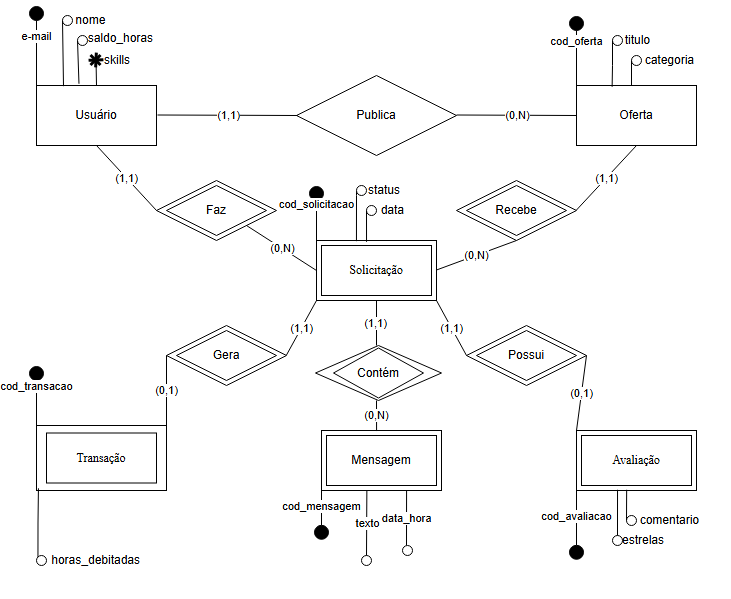
\includegraphics[width=0.52\textwidth]{der-tempus.png}
\caption{Representação das regras de negócio e relacionamentos.}
\end{figure}
\end{frame}

\begin{frame}
\frametitle{Modelo Físico - Estrutura de Tabelas}
\begin{figure}[htb!]
\centering
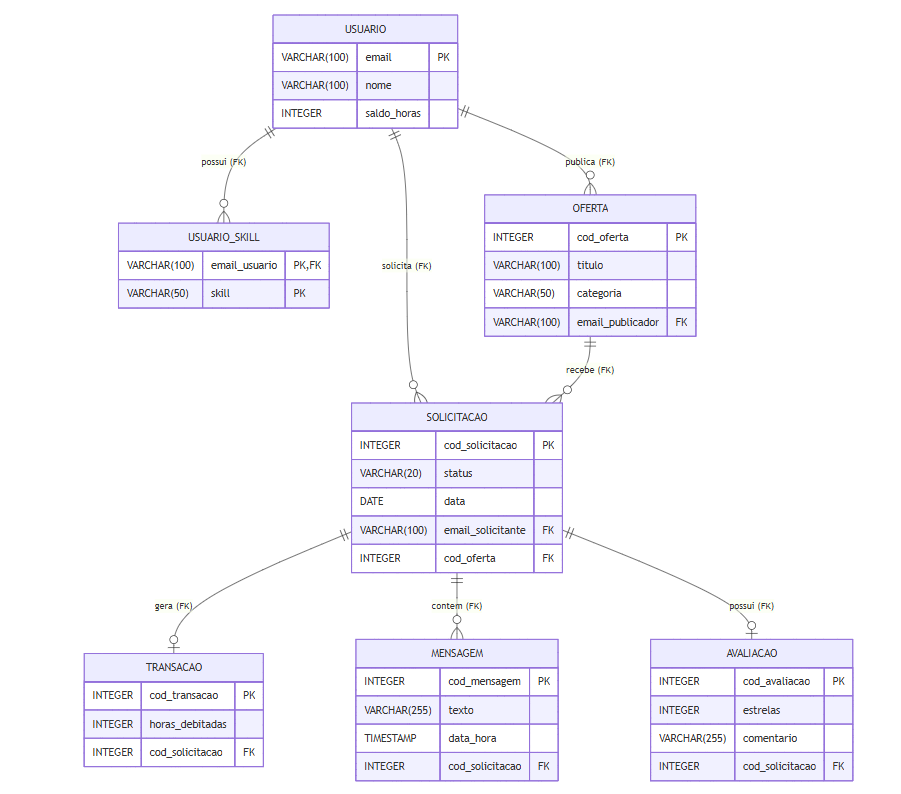
\includegraphics[width=0.48\textwidth]{der-fisico-tempus.png}
\caption{Implementação relacional com definição de chaves e tipos.}
\end{figure}
\end{frame}

%----
\section[Prototipação]{Prototipação}
%----

\begin{frame}
\frametitle{Protótipo: Menu Principal}
\begin{figure}
\centering
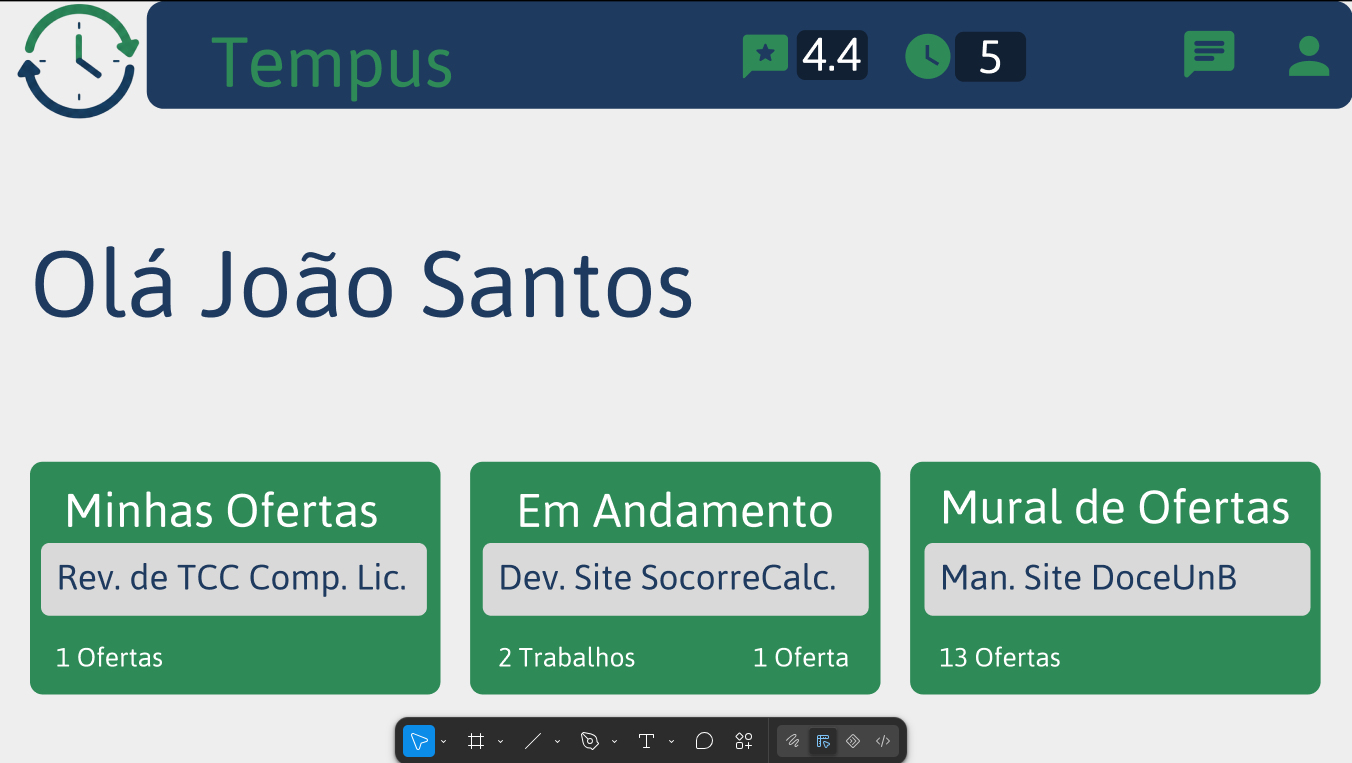
\includegraphics[width=0.85\linewidth]{menu-principal.png}
\end{figure}
\end{frame}

\begin{frame}
\frametitle{Protótipo: Chats}
\begin{figure}
    \centering
    \begin{minipage}{0.7\textwidth}
        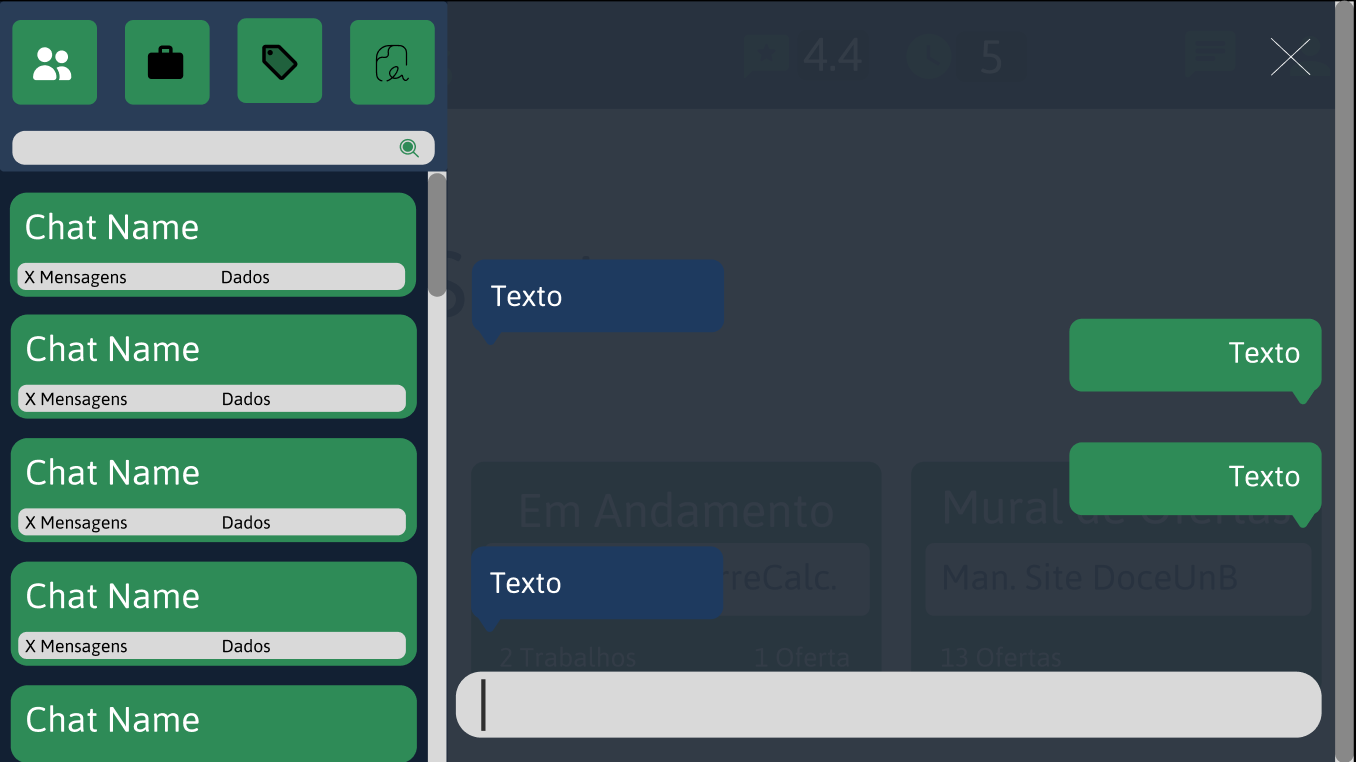
\includegraphics[width=1\linewidth]{chat-amigos.png}
    \end{minipage}
    \begin{minipage}{0.2\textwidth}
        
\includegraphics[width=0.8\linewidth]{chat-trabalhos.png}
        
\includegraphics[width=0.8\linewidth]{chat-ofertas.png}
        
\includegraphics[width=0.8\linewidth]{chat-negociçao.png}
    \end{minipage}
    \label{fig:my_label}
    \centering
\caption{Interface dos chats.}
\end{figure}
\end{frame}

\begin{frame}
\frametitle{Conexão: Protótipo, Requisitos e Dados}
\begin{itemize}
    \item RF11: Créditos Disponíveis
    \item RF13: Avaliações Recebidas
    \item RF16: Chats
    \item RF17: Notificações
\end{itemize}
\end{frame}

\begin{frame}
\frametitle{Protótipo: Perfil de Usuário}
\begin{figure}
\centering
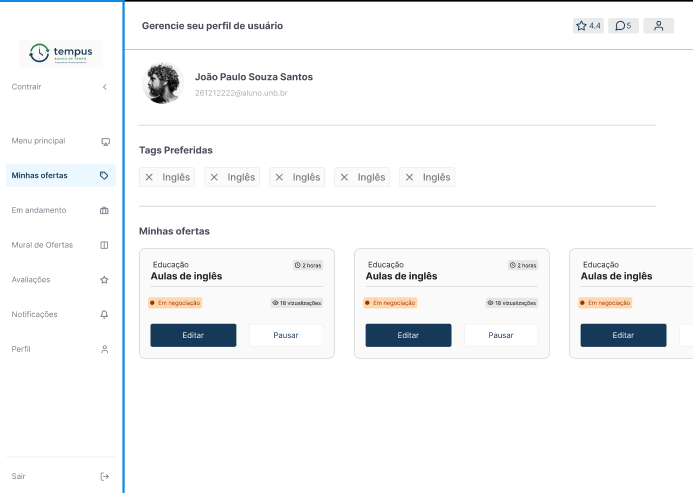
\includegraphics[width=0.8\linewidth]{perfil-de-usuario.png}
\end{figure}

\end{frame}
\begin{frame}
\frametitle{Conexão: Protótipo, Requisitos e Dados}
\begin{itemize}
    \item RF2: Perfil de Habilidades
    \item RF3: Gestão de Demandas
    \item RF13: Avaliações Recebidas
\end{itemize}
\end{frame}


\begin{frame}
\frametitle{Protótipo: Mural de Ofertas}

\begin{figure}
\centering

\begin{minipage}{0.39\textwidth}
\centering
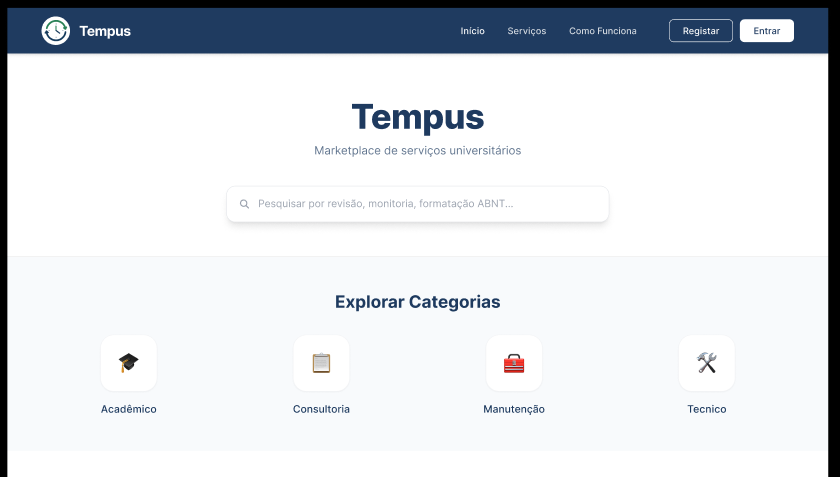
\includegraphics[width=\linewidth]{mural-ofertas-1.png}
\end{minipage}
\hfill
\begin{minipage}{0.39\textwidth}
\centering
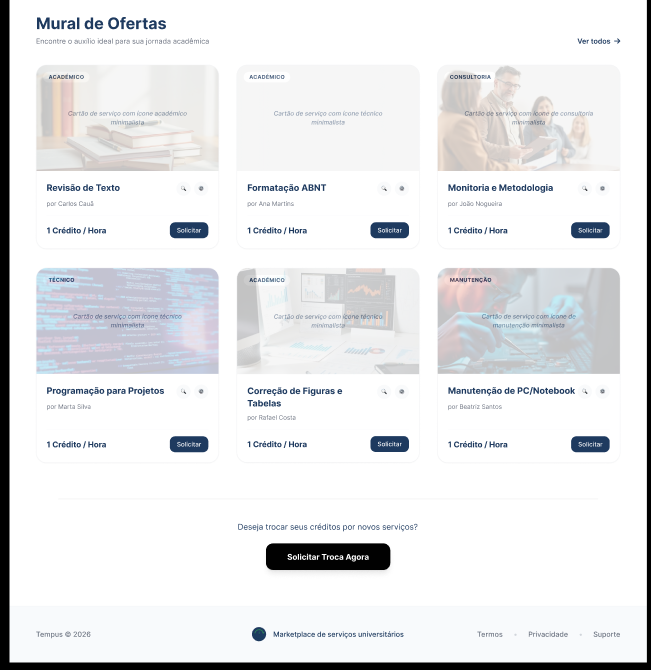
\includegraphics[width=\linewidth]{mural-ofertas-2.png}
\end{minipage}

\caption{Interfaces do Marketplace desenvolvidas no Figma.}
\end{figure}

\end{frame}

\begin{frame}
\frametitle{Conexão: Protótipo, Requisitos e Dados}
\begin{itemize}
    \item \textbf{RF04 e RF05 (Filtros e Busca):} A barra de pesquisa e botões interagem com a tabela \textit{OFERTA}, filtrando pelo atributo \texttt{categoria}.
    \item \textbf{RF06 (Mural Ativo):} Os cartões cruzam dados da \textit{OFERTA} com o \textit{USUARIO} (através da FK \texttt{email\_publicador}) para exibir o nome do prestador.
    \item \textbf{RF07 (Solicitação de Serviço):} O botão "Solicitar" é o gatilho que cria uma nova instância na entidade fraca \textit{SOLICITACAO}, unindo quem pede ao serviço ofertado.
\end{itemize}
\end{frame}



%------------------------------------------------
\section[Trabalhos em Andamento]{Trabalhos em Andamento}
%------------------------------------------------

% Slide 0
\begin{frame}
\vfill
\centering
{\Huge\textbf{Trabalhos em andamento}}
\vfill
\end{frame}

\begin{frame} 

\frametitle{Protótipo: Interface -- Minhas Ofertas} 

\small 

  

\textbf{Visão Geral} 

\begin{itemize} 

    \item \textbf{Objetivo:} Central de gerenciamento do portfólio pessoal do usuário. 

    \item \textbf{Diferencial:} Foco na autonomia para editar, pausar ou excluir serviços próprios. 

    \item \textbf{Funcionalidade:} Visão clara do "extrato de produtividade" e saldo de horas dentro do ecossistema Tempus. 

\end{itemize} 

  

\vspace{0.2cm} 

\textbf{Arquitetura da Informação} 

\begin{itemize} 

    \item \textbf{Métricas de Controle:} Resumo no topo com Total de Ofertas, Ofertas Ativas e Em Negociação. 

    \item \textbf{Filtros Dinâmicos:} Navegação rápida entre categorias de status para facilitar a busca interna. 

    \item \textbf{Ação Primária:} Botão "+ Nova Oferta" posicionado no topo para incentivar a criação de novos serviços. 

\end{itemize} 

  

\vspace{0.2cm} 

\textbf{Anatomia do Card de Serviço} 

\begin{itemize} 

    \item \textbf{Identificação:} Título do serviço e carga horária (unidade de troca). 

    \item \textbf{Gestão Direta:} Inclusão do botão "Editar" em cada módulo, garantindo agilidade sem necessidade de menus complexos. 

\end{itemize} 

  

\end{frame} 
% Slide 1
\begin{frame}
\frametitle{Cabeçalho padrão do Tempus}
\begin{figure}
\centering
\includegraphics[width=0.96\linewidth,height=0.78\textheight,keepaspectratio]{\detokenize{Slide 1 - Cabeçalho padrão do Tempus.png}}
\end{figure}
\end{frame}

% Slide 2
\begin{frame}
\frametitle{RF6 — Indicador de Reputação}
\begin{figure}
\centering
\includegraphics[width=0.96\linewidth,height=0.78\textheight,keepaspectratio]{\detokenize{Slide - RF6 - Indicador de Reputação.png}}
\end{figure}
\end{frame}

% Slide 3
\begin{frame}
\frametitle{RF4 e US07 — Carteira de Créditos}
\begin{figure}
\centering
\includegraphics[width=0.96\linewidth,height=0.78\textheight,keepaspectratio]{\detokenize{Slide 3 - RF4 e US07 - Carteira de Créditos.png}}
\end{figure}
\end{frame}

% Slide 4
\begin{frame}
\frametitle{RF7 — Chat Interno}
\begin{figure}
\centering
\includegraphics[width=0.96\linewidth,height=0.78\textheight,keepaspectratio]{\detokenize{Slide 4 - RF7 - Chat Interno.png}}
\end{figure}
\end{frame}

% Slide 5
\begin{frame}
\frametitle{RNF2 — Título e Subtítulo}
\begin{figure}
\centering
\includegraphics[width=0.96\linewidth,height=0.78\textheight,keepaspectratio]{\detokenize{Slide 5 - RNF2 - Título e subtítulo.png}}
\end{figure}
\end{frame}

% Slide 6
\begin{frame}
\frametitle{Seção das Abas}
\begin{figure}
\centering
\includegraphics[width=0.96\linewidth,height=0.78\textheight,keepaspectratio]{\detokenize{Slide 6 - Seção das abas.png}}
\end{figure}
\end{frame}

% Slide 7
\begin{frame}
\frametitle{RF3 — Solicitados, Em andamento e Aguardando confirmação}
\begin{figure}
\centering
\includegraphics[width=0.96\linewidth,height=0.78\textheight,keepaspectratio]{\detokenize{Slide 7 - RF3 - Solicitados, Em andamento, Aguardando confirmação.png}}
\end{figure}
\end{frame}

% Slide 8
\begin{frame}
\frametitle{RF5 — Concluídos}
\begin{figure}
\centering
\includegraphics[width=0.96\linewidth,height=0.78\textheight,keepaspectratio]{\detokenize{Slide 8 - RF5 - Concluídos.png}}
\end{figure}
\end{frame}

% Slide 9
\begin{frame}
\frametitle{RF8 — Em disputa}
\begin{figure}
\centering
\includegraphics[width=0.96\linewidth,height=0.78\textheight,keepaspectratio]{\detokenize{Slide 9 - RF8 - Em disputa.png}}
\end{figure}
\end{frame}

% Slide 10
\begin{frame}
\frametitle{Cartões}
\begin{figure}
\centering
\includegraphics[width=0.96\linewidth,height=0.78\textheight,keepaspectratio]{\detokenize{Slide 10 - Cartões.png}}
\end{figure}
\end{frame}

% Slide 11
\begin{frame}
\frametitle{RR1 — Serviços no contexto acadêmico}
\begin{figure}
\centering
\includegraphics[width=0.96\linewidth,height=0.78\textheight,keepaspectratio]{\detokenize{Slide 11 - RR1 - Serviços.png}}
\end{figure}
\end{frame}

% Slide 12
\begin{frame}
\frametitle{RF3 — Solicitante e prestador}
\begin{figure}
\centering
\includegraphics[width=0.96\linewidth,height=0.78\textheight,keepaspectratio]{\detokenize{Slide 12 - RF3 - Solicitante e prestador.png}}
\end{figure}
\end{frame}

% Slide 13
\begin{frame}
\frametitle{RF5 e RR3 — Data, duração e valor da troca}
\begin{figure}
\centering
\includegraphics[width=0.96\linewidth,height=0.78\textheight,keepaspectratio]{\detokenize{Slide 13 - RF5 e RR3 - Data combinada, duração estimada e valor da troca.png}}
\end{figure}
\end{frame}

% Slide 14
\begin{frame}
\frametitle{RF3 e US06 — Status}
\begin{figure}
\centering
\includegraphics[width=0.96\linewidth,height=0.78\textheight,keepaspectratio]{\detokenize{Slide 14 - RF3 e US06 - Status.png}}
\end{figure}
\end{frame}

% Slide 15
\begin{frame}
\frametitle{RF7 — Abrir chat}
\begin{figure}
\centering
\includegraphics[width=0.96\linewidth,height=0.78\textheight,keepaspectratio]{\detokenize{Slide 15 - RF7 - Abrir chat.png}}
\end{figure}
\end{frame}

% Slide 16
\begin{frame}
\frametitle{RF3 e US06 — Confirmar conclusão}
\begin{figure}
\centering
\includegraphics[width=0.96\linewidth,height=0.78\textheight,keepaspectratio]{\detokenize{Slide 16 - RF3 e US06 - Confirmar conclusão.png}}
\end{figure}
\end{frame}

% Slide 17
\begin{frame}
\frametitle{RF8 e RNF5 — Abrir disputa}
\begin{figure}
\centering
\includegraphics[width=0.96\linewidth,height=0.78\textheight,keepaspectratio]{\detokenize{Slide 17 - RF8 e RNF5 - Abrir disputa.png}}
\end{figure}
\end{frame}

% Slide 18
\begin{frame}
\frametitle{RF5 — Ver detalhes}
\begin{figure}
\centering
\includegraphics[width=0.96\linewidth,height=0.78\textheight,keepaspectratio]{\detokenize{Slide 18 - RF5 - Ver detalhes.png}}
\end{figure}
\end{frame}

% Slide 19
\begin{frame}
\frametitle{Síntese da tela}
\small
\begin{itemize}
    \item A organização visual da tela contribui para o \textbf{RNF2 — Usabilidade}, com cartões, filtros, cores, ícones e textos objetivos.
    \item A tela representa o \textbf{RR6}, pois o Tempus foi planejado como uma aplicação web.
    \item Também atende ao \textbf{RR9}, pois o acesso foi pensado para navegadores modernos, sem instalação local.
    \item A tela atende principalmente aos requisitos \textbf{RF3, RF4, RF5, RF6, RF7 e RF8}.
    \item Além disso, contribui para \textbf{RNF2, RNF5, RR1, RR3, RR6 e RR9}.
\end{itemize}
\end{frame}

%------------------------------------------------
\begin{frame}
\Large{\centerline{Obrigado Pela Atenção!}}
\Large{\centerline{Perguntas?}}
\end{frame}
%------------------------------------------------
\end{document}
